\newcommand{\duedate}{22 October 2026}
\documentclass{16384_doc}
\usepackage{enumitem}
\usepackage{tikz}
\usetikzlibrary{positioning,arrows,arrows.meta,matrix,fit,backgrounds,calc,math,patterns,patterns.meta,intersections,fpu}
\newcommand{\assignmentname}{Assignment 5: 2D Lagrangian Dynamics}

\begin{document}
\maketitle

\tableofcontents

\section{Theory Questions}

\begin{questions}
    \titledquestion{Spring, cart, pendulum}[30]

    The following spring-cart-pendulum system shown below is a modification of the pendulum-cart discussed in class. The cart has mass $M$, the pendulum has mass $m$ and its spring has rest length $r_0$ and spring constant $k$.
    \begin{center}
        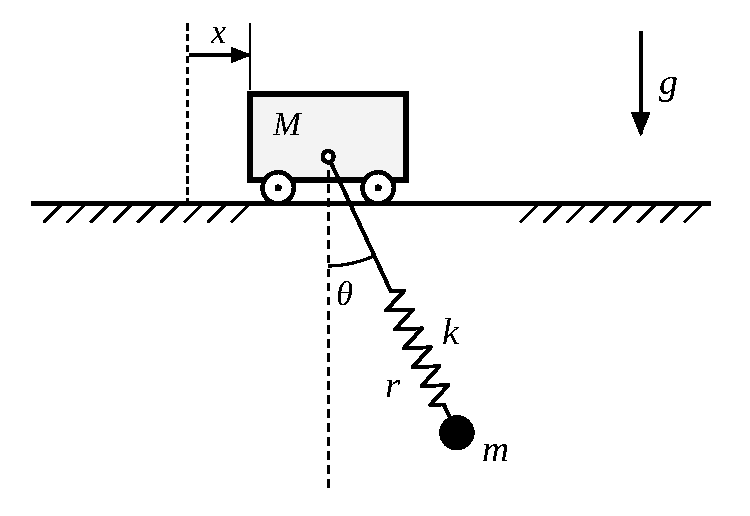
\includegraphics[width=0.4\textwidth]{generated_figures/cart_pendulum_spring.pdf}
    \end{center}

    \begin{enumerate}[label=\alph*.]
        \item \text{[10 points]} Write the potential and kinetic energy of the system in terms of the generalized coordinates $q = [x, r, \theta]^\top$ and their time derivatives $\dot q = [\dot x, \dot r, \dot\theta]^\top$. Then write the Lagrangian of the system.
        \begin{tcolorbox}[height=4cm]
            % TODO: ENTER YOUR ANSWER HERE
        \end{tcolorbox}

        \item \text{[10 points]} Write the derivatives of $\mathcal L$ with respect to $q$ and $\dot q$ (6 in total).
        \begin{tcolorbox}[height=6cm]
            % TODO: ENTER YOUR ANSWER HERE
        \end{tcolorbox}

        \pagebreak
        \item \text{[5 points]} Write the equations of motion of the system using the Euler-Lagrange equations.
        \begin{tcolorbox}[height=3cm]
        \end{tcolorbox}

        \item \text{[5 points]} Suppose you can control the cart with an external force $f_x$. Write the equations of motion with the control input $f_x$.
        \begin{tcolorbox}[height=3cm]
        \end{tcolorbox}
    \end{enumerate}

    \pagebreak
    \titledquestion{Double Pendulum}[30]
    The double pendulum is a classic example of a chaotic system, yet its equations of motion are relatively simple to derive. You will be using your derived equations of motion to simulate the double pendulum in the coding section of this assignment.

    The masses $m_1$ and $m_2$ are point masses at the ends of massless rods of length $\ell_1$ and $\ell_2$. Both angles are measured from the downward vertical, as shown in the figure: $\theta_2$ is the absolute angle of link 2, \emph{not} its angle relative to link 1. Gravity points in the $-y$ direction.

    \begin{center}
        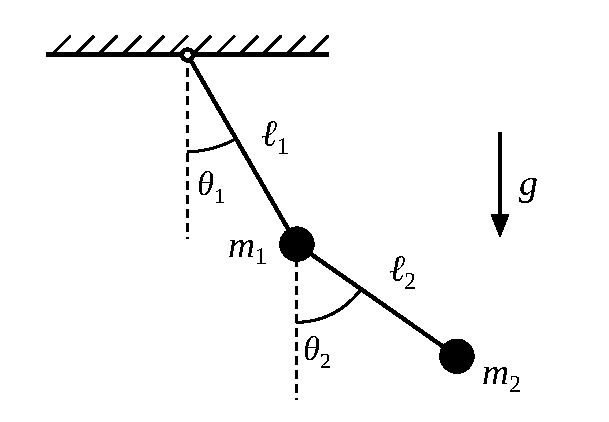
\includegraphics[width=0.4\textwidth]{generated_figures/double_pendulum.pdf}
    \end{center}
    
    \begin{enumerate}[label=\alph*.]
        \item \text{[10 points]} Write the potential and kinetic energy of the system in terms of the generalized coordinates $q = [\theta_1, \theta_2]^\top$ and their time derivatives $\dot q = [\dot \theta_1, \dot \theta_2]^\top$.
        \begin{tcolorbox}[height=4cm]
        \end{tcolorbox}

        \item \text{[10 points]} Write the derivatives of $\mathcal L$ with respect to $q$ and $\dot q$ (4 in total).
        \begin{tcolorbox}[height=6cm]
        \end{tcolorbox}

        \pagebreak
        \item \text{[10 points]} Write the equations of motion of the system using the Euler-Lagrange equations.
        \begin{tcolorbox}[height=3cm]
        \end{tcolorbox}
    \end{enumerate}

    \pagebreak
    \titledquestion{RRR Arm Dynamics}[40]

    Consider the following robot. Assume no joint limits, and that the links lengths are $l_1=l_2=l_3=1$, and the masses are $m_1=m_2=m_3=1$. The joint angles are measured as a relative angle from the previous link / horizontal, so $\th[1]=\th[2]=\th[3]=0$ means the arm is fully extended to the right. Each link's mass is spread uniformly along its length, so its center of mass is at its midpoint and its moment of inertia about its center of mass is $I_i = \frac{1}{12} m_i l_i^2 = \frac{1}{12}$. Gravity points in the $-y$ direction.
    \begin{center}
        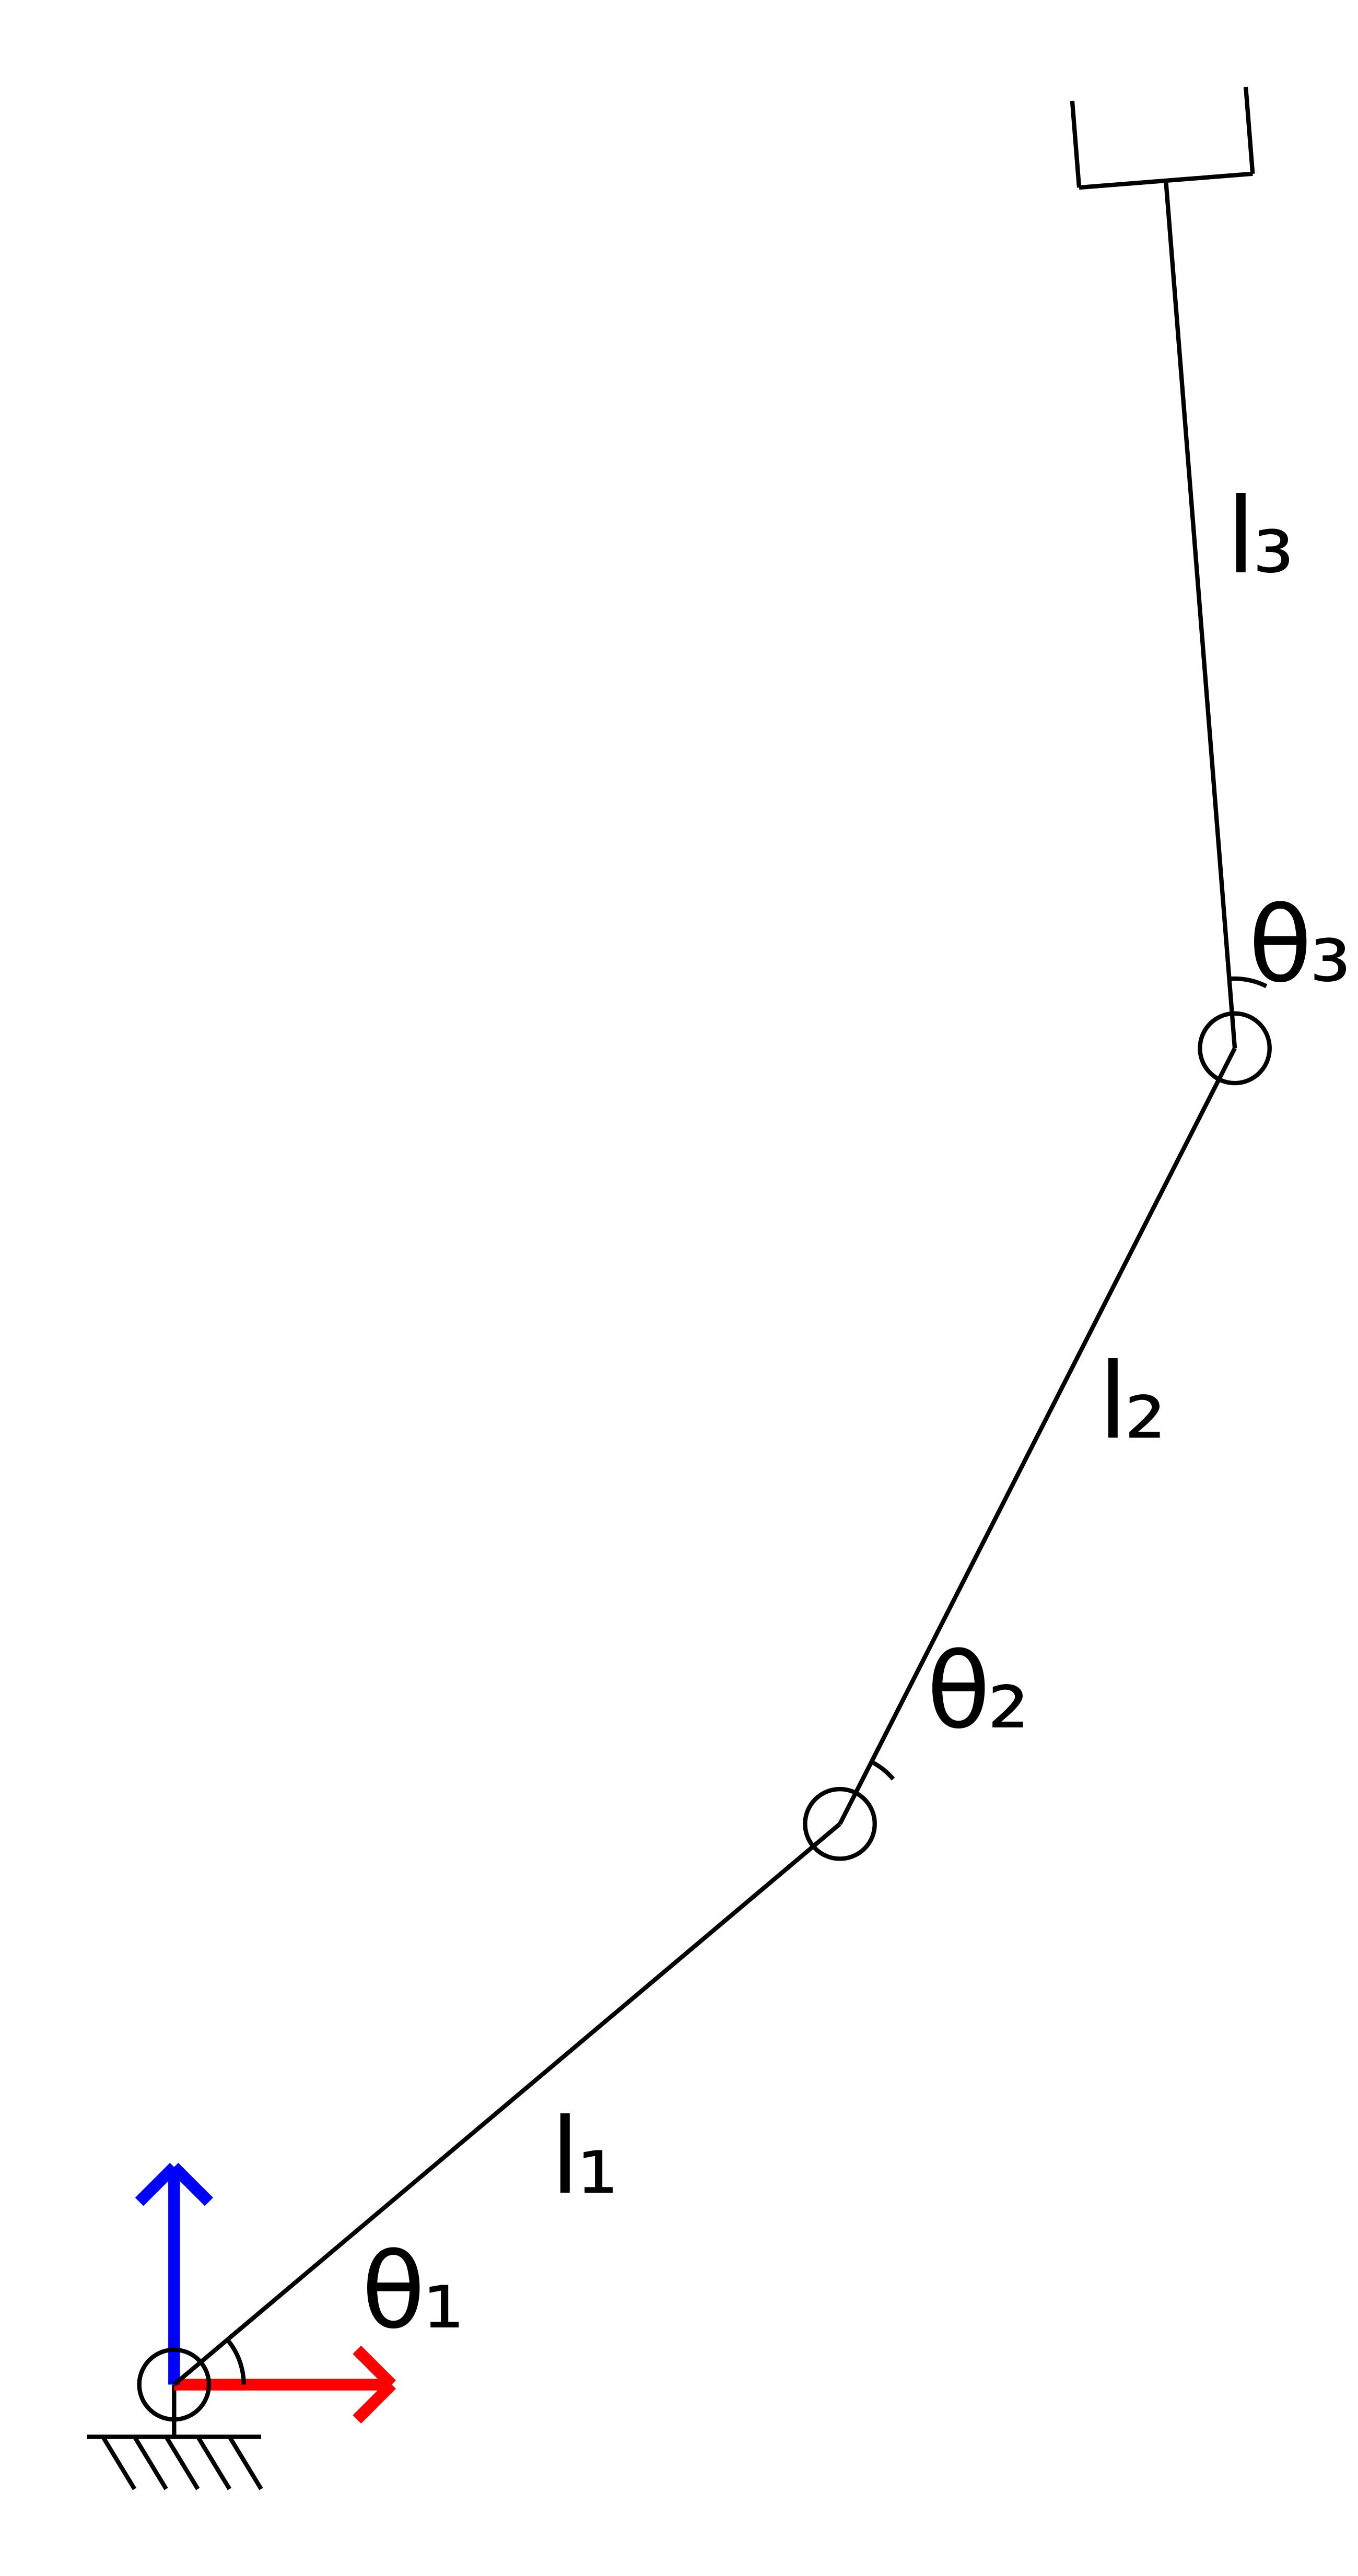
\includegraphics[scale=0.07]{generated_figures/robot_1.png}
    \end{center}

    \begin{enumerate}[label=\alph*.]
        \item \text{[10 points]} Write the potential and kinetic energy of the system in terms of the generalized coordinates $q = [\theta_1, \theta_2, \theta_3]^\top$ and their time derivatives $\dot q = [\dot \theta_1, \dot \theta_2, \dot \theta_3]^\top$.
        \begin{tcolorbox}[height=4cm]
        \end{tcolorbox}

        \pagebreak
        \item \text{[10 points]} Write the derivatives of $\mathcal L$ with respect to $q$ and $\dot q$ (6 in total).
        \begin{tcolorbox}[height=6cm]
        \end{tcolorbox}

        \item \text{[10 points]} Write the equations of motion of the system using the Euler-Lagrange equations. Include external torques $\tau_1, \tau_2, \tau_3$ applied at each joint.
        \begin{tcolorbox}[height=3cm]
        \end{tcolorbox}

        \item \text{[5 points]} Find the standard form matrices $M(q)$, $C(q, \dot q)$, and $G(q)$ such that the equations of motion can be written as $M(q)\ddot q + C(q, \dot q)\dot q + G(q) = \tau$.
        \begin{tcolorbox}[height=3cm]
        \end{tcolorbox}

        \item \text{[5 points]} What are the joint torques $\tau_1, \tau_2, \tau_3$ required to hold the arm in the configuration $\theta_1 = \theta_2 = \theta_3 = 0$ (fully extended to the right) with no motion? How does this compare to the Jacobian-based gravity compensation method discussed previously?
        \begin{tcolorbox}[height=3cm]
        \end{tcolorbox}
    \end{enumerate}


\end{questions}

% \section{Code Questions}

% \begin{questions}
%     \setcounter{question}{3}
%     \titledquestion{Double Pendulum Simulation}[45]
%     In this question you will simulate the double pendulum from the written section using the equations of motion you derived. All the code is in the \verb!code/! folder; \verb!code/README.md! explains how to run each script. You edit and submit only \verb!double_pendulum.py!.

%     Use the same conventions as the written section: $q = [\theta_1, \theta_2]^\top$ with both angles measured from the downward vertical (counterclockwise positive), and point masses $m_1, m_2$ on massless links $\ell_1, \ell_2$. There is no applied torque in the code ($\tau = 0$). In your code, use the constants \verb!M1!, \verb!M2!, \verb!L1!, \verb!L2! and \verb!G! at the top of \verb!double_pendulum.py! rather than writing the numbers in directly, because the autograder changes them.

%     \begin{enumerate}[label=\alph*.]
%         \item \text{[20 points]} Implement \verb!dynamics(q, qd)!, which returns the joint accelerations $\ddot q$ as an array of shape $(2,)$. Your Euler-Lagrange equations are linear in $\ddot q$, so write them as $M(q)\ddot q = b(q, \dot q)$ and solve for $\ddot q$ with \verb!np.linalg.solve!.

%         \item \text{[15 points]} Implement \verb!simulate(q0, qd0, T, dt)!. We recommend using a library like \verb!scipy.integrate.solve_ivp! to integrate the equations of motion with the supplied \verb|RTOL| and \verb|ATOL| tolerances, but also encourage you to try implementing your own integrator to learn a little about numerical integration. You'll see the difference in (c).

%         The output format should be a tuple \verb!(t, q, qd)! of numpy arrays, sampled every \verb!dt! seconds from $0$ to $T$ inclusive (use \verb!np.arange(0, T + dt / 2, dt)!, so there are $N = T/\Delta t + 1$ samples):
%         \begin{itemize}
%             \item \verb!t!: the sample times $0, \Delta t, 2\Delta t, \dots, T$, shape $(N,)$.
%             \item \verb!q!: the joint angles $[\theta_1, \theta_2]$ at each sample time, shape $(N, 2)$.
%             \item \verb!qd!: the joint velocities $[\dot\theta_1, \dot\theta_2]$ at each sample time, shape $(N, 2)$.
%         \end{itemize}
%         The first row of \verb!q! and \verb!qd! is the initial state \verb!q0!, \verb!qd0!.

%         Run \verb!python autograder.py! to check parts (a) and (b), then watch your pendulum with \verb!python visualize.py!.

%         \item \text{[5 points]} With no friction and no applied torque, the total energy $E = T + V$ of the double pendulum stays constant. That gives you a way to check a simulation without knowing the right answer: if $E$ changes over time, the simulation is not exactly following the physics.

%         Implement \verb!total_energy(q, qd)! in \verb!double_pendulum.py! using your $T$ and $V$ from the written section (the autograder checks it too). Then run \verb!python energy_check.py!, which simulates the pendulum for 20 seconds and plots its total energy over time.

%         Does your simulation conserve energy? If the energy changes noticeably, what could cause it?
%         \begin{tcolorbox}[height=3cm]
%         \end{tcolorbox}

%         \item \text{[5 points]} Run \verb!python visualize.py --chaos 5 --plot!, which simulates five pendulums whose starting $\theta_2$ values differ by only $0.001$ rad. About how long do the pendulums stay together before they visibly separate? Now try a small initial angle, \verb!python visualize.py --chaos 5 --q0 10 5!. Is the motion still chaotic? Explain the difference.
%         \begin{tcolorbox}[height=3cm]
%         \end{tcolorbox}
%     \end{enumerate}
% \end{questions}

\begin{submissionChecklist}
        \item Create a PDF of your answers to the written questions with the name \verb!<andrew_id>.pdf! and submit it to Gradescope.
        % \item Run \verb!autograder.py! and confirm it reports no failures.
        % \item Run \verb!create_submission.py! in the python terminal.
        % \item Rename \verb|submission.zip| and upload \verb!<andrew_id>.zip! to Gradescope.
        % \item Coding questions are autograded, with no limit on number of submissions within the mandated deadline.
\end{submissionChecklist}

\end{document}
